\documentclass[11pt,a4paper]{article}
\usepackage[utf8]{inputenc}\usepackage[T1]{fontenc}
\usepackage[margin=1in]{geometry}
\usepackage{amsmath,amssymb,booktabs,graphicx,enumitem,xcolor,parskip,titlesec}
\usepackage[hidelinks]{hyperref}
\graphicspath{{figures/}}
\definecolor{qnavy}{RGB}{20,40,75}\definecolor{qgrey}{RGB}{90,90,90}
\titleformat{\section}{\large\bfseries\color{qnavy}}{\thesection}{0.6em}{}
\begin{document}\thispagestyle{empty}
\noindent
{\large\bfseries\color{qnavy} Report R03 --- FASN and the Lipogenic Phenotype in HCC}\\[2pt]
{\color{qgrey}Independent test of the withdrawn manuscript's three claims.}\\[6pt]
{\color{qgrey}\rule{\textwidth}{0.4pt}}

\medskip
\noindent 7 August 2026 \quad\textbullet\quad Quantara

\section*{Summary}

The withdrawn HCC manuscript claimed FASN associates with tumour stage, vascular invasion
and survival. We tested all three in the Chinese Liver Cancer Atlas (238 RNA-sequenced
tumours), a cohort independent of the TCGA-LIHC data in which those claims previously
failed. \textbf{None of the three associations is present} after multiplicity correction.

What \emph{does} replicate is the lipogenic phenotype itself: FASN co-expresses tightly with
ACACA ($\rho=+0.546$), SCD ($+0.510$) and SREBF1 ($+0.495$), all $p<4\times10^{-16}$.

A pre-registered positive control confirms the analysis is sound rather than merely
negative: AFP gene expression correlates with the independently measured serum AFP
concentration at $\rho=0.667$, $p=5.5\times10^{-32}$ --- two different assays of the same
biology, agreeing strongly. The clinical join and the expression matrix are therefore
verified.

\section{Results}

\begin{center}
\begin{tabular}{@{}lccc@{}}
\toprule
\textbf{Test} & \textbf{Statistic} & \textbf{$p$} & \textbf{$q$ (BH)} \\
\midrule
\multicolumn{4}{@{}l}{\itshape Positive control} \\
AFP expression vs serum AFP ($n=238$) & $\rho=0.667$ & $5.5\times10^{-32}$ & --- \\
\midrule
\multicolumn{4}{@{}l}{\itshape Lipogenic co-expression (replication)} \\
FASN $\sim$ ACACA & $\rho=+0.546$ & $7.1\times10^{-20}$ & --- \\
FASN $\sim$ SCD & $\rho=+0.510$ & $3.8\times10^{-17}$ & --- \\
FASN $\sim$ SREBF1 & $\rho=+0.495$ & $3.9\times10^{-16}$ & --- \\
\midrule
\multicolumn{4}{@{}l}{\itshape The manuscript's claims} \\
Vascular invasion (M0/M1/M2, $n=237$) & $H=1.80$ & 0.407 & 0.509 \\
\quad absent vs present & --- & 0.201 & --- \\
BCLC stage & $H=1.62$ & 0.656 & 0.656 \\
Edmondson grade & $H=2.39$ & 0.122 & 0.299 \\
Survival status (living vs deceased, $n=183$) & --- & 0.179 & 0.299 \\
Recurrence status ($n=183$) & --- & 0.072 & 0.299 \\
\bottomrule
\end{tabular}
\end{center}

\begin{center}
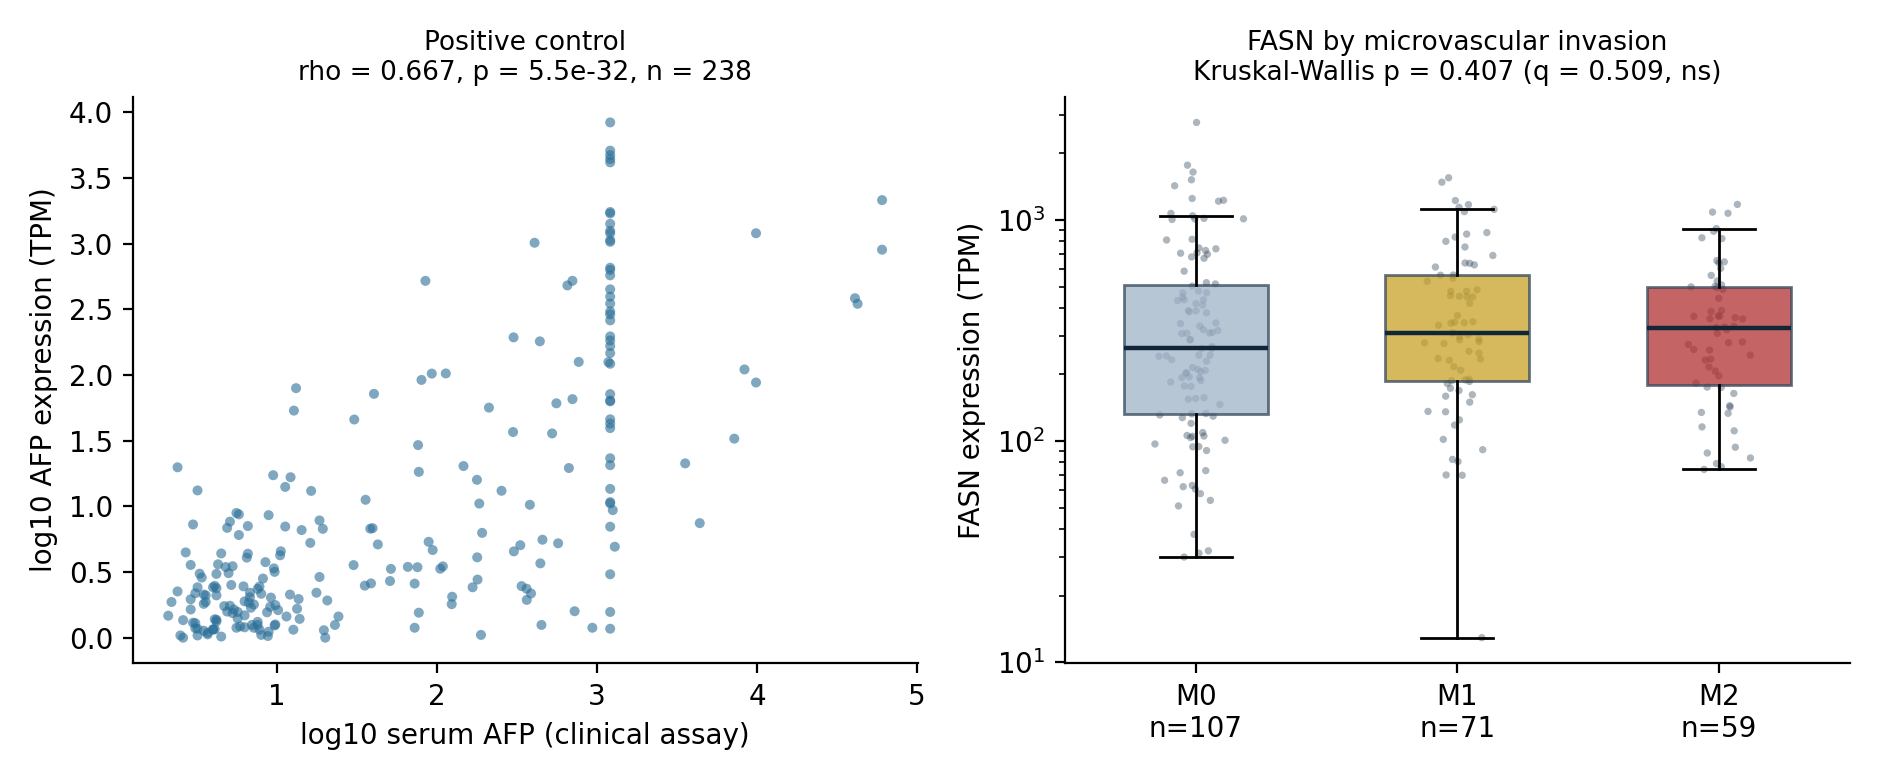
\includegraphics[width=\textwidth]{fig1_control_and_mvi.png}
\end{center}

\section{Interpretation, with the nuance the numbers require}

\textbf{The lipogenic phenotype is real.} FASN sits in a coherently co-regulated lipogenic
programme, replicated here and previously in TCGA-LIHC ($\rho=+0.62$, $+0.62$, $+0.42$).
That part of the manuscript survives.

\textbf{The clinical associations do not.} Two independent cohorts now agree: FASN
expression does not track stage, vascular invasion or outcome.

\textbf{But this is absence of evidence for a \emph{small} effect, not proof of no effect.}
The audit quantified what we could have detected. For vascular invasion absent versus
present, the minimum detectable rank-biserial correlation at 80\% power is 0.212; the
observed value is 0.097. So a moderate or larger association is excluded, while a small one
is not. The report should not claim more than that.

\textbf{One honest complication.} Median FASN rises monotonically across invasion grades
(262.7 $\to$ 308.7 $\to$ 326.1 TPM), which is the direction the manuscript predicted. The
means do not (423 $\to$ 434 $\to$ 383), the test is null, and the effect is below the
detectable threshold. We mention the trend because omitting it would be selective, not
because it supports the claim.

\section{Audit}

\begin{center}
\begin{tabular}{@{}llp{7.6cm}@{}}
\toprule
\textbf{Check} & \textbf{Verdict} & \textbf{Finding} \\
\midrule
Positive control & \textbf{Strong} & $\rho=0.667$ between two independent AFP assays; join and matrix verified \\
Power for the null & \textbf{Quantified} & Observed effect 0.097 vs minimum detectable 0.212 --- small effects not excluded \\
Censored inputs & \textbf{Handled} & 43 of 238 serum AFP values are `$>$' or `$<$' capped; rank-based tests are unaffected in ordering \\
Expression sanity & \textbf{Plausible} & FASN 12.9--2763.5 TPM, median 304.6, no zeros \\
Gates & \textbf{6 / 6 PASS} & Sample count, gene presence, clinical join, control, replication \\
\bottomrule
\end{tabular}
\end{center}

\section{Consequence for the HCC manuscript}

The revised manuscript should report the lipogenic co-expression phenotype and state
plainly that FASN showed no association with stage, vascular invasion, grade, survival
status or recurrence in either of two independent cohorts, with the power limitation
stated. Combined with the earlier finding that FASN protein is \emph{lower} in tumour while
JUN protein is higher, and that no resolvable locus exists for the transcript designated
HELC, the honest position is a descriptive biomarker report with an explicitly negative
mechanistic result.

\section{How to verify}

\texttt{evidence/fasn\_by\_sample.csv} carries FASN TPM, AFP TPM and serum AFP for all 238
samples, so the positive control and every FASN test can be recomputed. Also included:
\texttt{config.yaml} (hash \texttt{f4da7e3d\ldots}, written before any outcome was read),
\texttt{gates.json}, \texttt{results.json} (all $p$ and $q$ values),
\texttt{audit\_power.json}, \texttt{inputs.json} (file hashes),
\texttt{MANIFEST.sha256}, \texttt{env.txt}, \texttt{m3\_hcc\_fasn.py}.

\vfill
\noindent{\color{qgrey}\rule{\textwidth}{0.4pt}}\\
{\footnotesize\color{qgrey}Run directory \texttt{runs/20260806T225833Z-R03hcc-3f8bece}.
Data: Chinese Liver Cancer Atlas via cBioPortal (\texttt{hcc\_clca\_2024}), Open Database
Licence. No patient-level identifiers reproduced.}
\end{document}
